\documentclass[12pt,a4paper]{article}
\usepackage[utf8]{inputenc}
\usepackage[german]{babel}
\usepackage[T1]{fontenc}
\usepackage{amsmath}
\usepackage{amsfonts}
\usepackage{amssymb}
\usepackage{graphicx}
\usepackage[left=2.5cm,right=2.5cm,top=2cm,bottom=2cm]{geometry}
\author{Gruppe C14 \\ Julián Häck, Martin Koytek, Lars Wenning, Erik Zimmermann}
\usepackage{subfigure}
\usepackage{float}
\begin{document}
\section{Gedämpfter LC Schwingkreis Oszilloskop, Teilversuch 4.4.1}
\subsection{Versuchsbeschreibung}
In diesem Versuch soll die Frequenz $f$ und der Dämpfungskoeffizient $\delta$ eines LRC-Schwingkreises mit Hilfe eines Oszilloskops bestimmt werden. \newline
Dazu wird die Spannung über dem Kondensator mit dem Oszilloskop aufgezeichnet, um die Frequenz und den Abklingkoeffizienten folgendermaßen zu bestimmen:
\begin{equation}
f=\frac{1}{t_{n+1}-t_n}=\frac{1}{\Delta t}
\end{equation}
\begin{equation}
\delta_n=\frac{\ln{(\frac{U_n}{U_{n+1}})}}{t_{n+1}-t_n}.
\end{equation}


\subsection{Versuchsaufbau und Durchführung}

\begin{figure}[H]
\centering
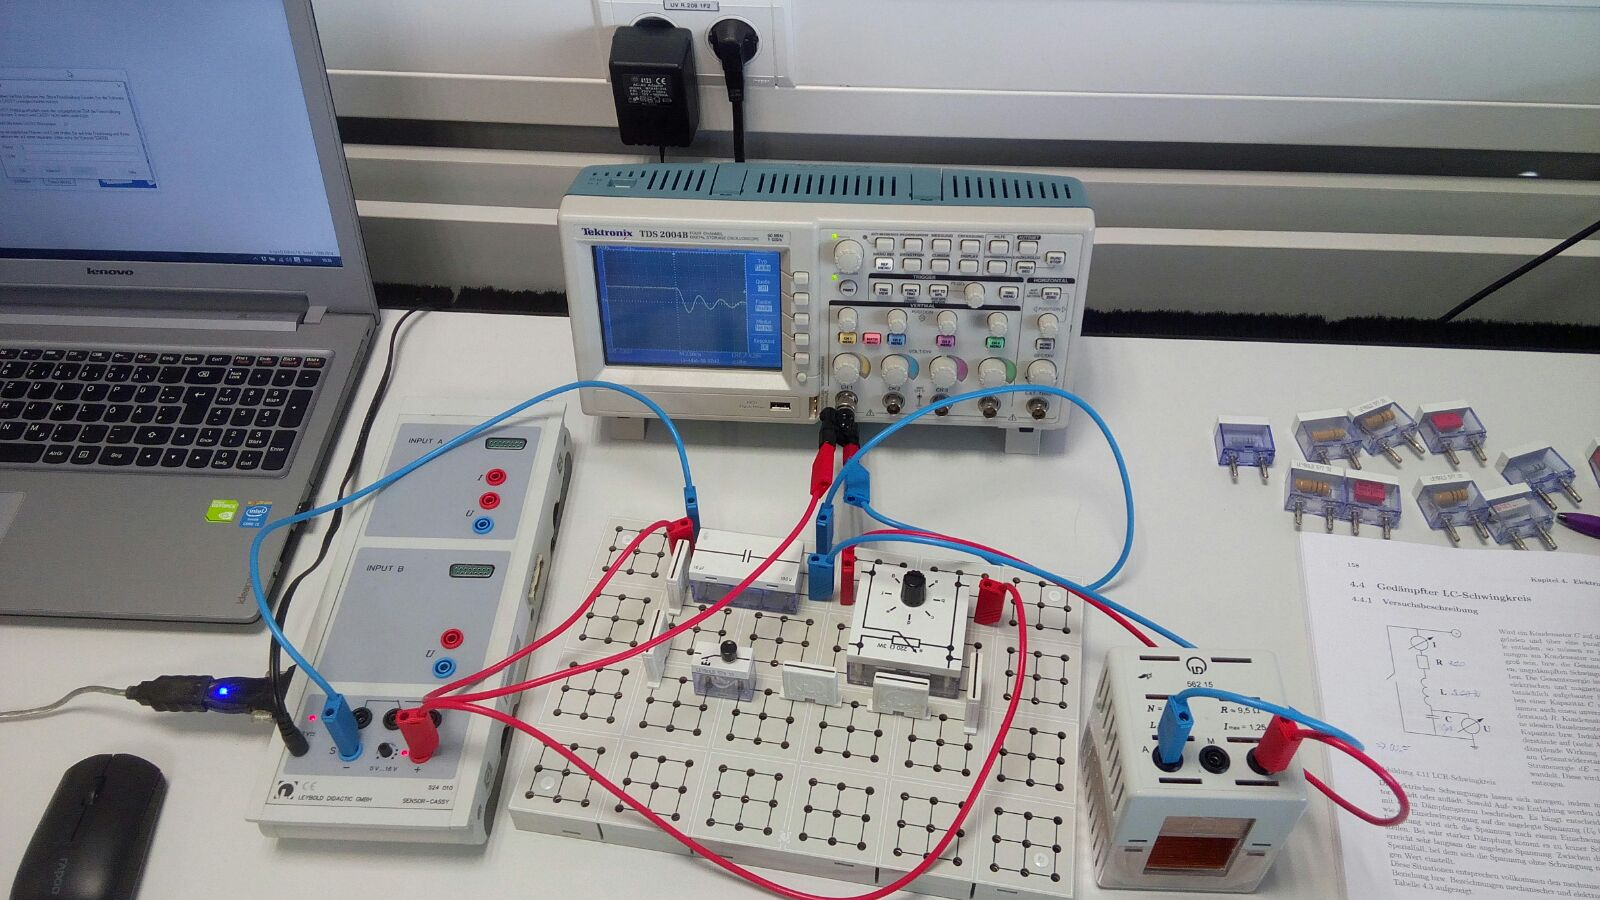
\includegraphics[scale=0.27]{ArbeitsplatzE_1.jpg}
\caption{Versuchsaufbau}
\end{figure}


\begin{itemize}
\item Bei dem oben gezeigten LRC Schwingkreis wurde der Drehwiderstand komplett herunter geregelt ($R=0.02\Omega$). Dieser wird erst später in Versuch 4.4.2 gebraucht.
 
\item Alle Versuche wurden bei einer Eingangspannung von $U_0=5.6V$ durchgeführt, dabei wurde das Oszilloskop auf \glqq Single Sequence\grqq $\,$ eingestellt und aus dem resultierenden Standbild die Spannungsmaxima mit entsprechenden Zeitwerten abgelesen. Dazu wurden die Messbereiche auf $U_B=16V$ (Spannung) \& $T_B=50 \cdot 10^{-3}s$ (Zeit) eingestellt.
\item Es lag ein Offset von $off=50 \cdot 10^{-3}V$ vor, der im Folgenden ausgeglichen wurde.
\item Die Ablesefehler wurden zu $\sigma_U=\frac{0.08}{\sqrt{12}}V$ \& $\sigma_T=\frac{100\cdot 10^{-6}}{\sqrt{12}}s$ bestimmt.
Diese Messung wurde 4 mal wiederholt wobei die Ergebnisse des 2. Versuchs aufgrund eines Stromausfalls verloren gingen.
\end{itemize}

\newpage
\subsection{Versuchsauswertung}

\subsubsection{Rohdaten}

Spule (Herstellerangaben): 
\begin{figure}[H]\centering
\begin{tabular}{c|l}
Induktivität & $L=36*10^{-3}H$\\ 
Windungen & $N=1000$\\ 
Widerstand & $R=9.5\Omega$ \\
\end{tabular} 
\end{figure}

Kondensator (Herstellerangabe):
\begin{figure}[H]\centering
\begin{tabular}{c|l}
Kapazität & $C=10*10^{-6}F$\\ 
\end{tabular} 
\end{figure}

Messdaten:
\begin{table}[H]\centering
\caption{1. Messung}
\begin{tabular}{c|c}
\hline
$U_1=3.12V$& $t_1=0.5ms$\\ 
$U_2=1.76V$& $t_2=4.4ms$\\ 
$U_3=1.04V$& $t_3=8.2ms$ \\
$U_4=0.56V$& $t_4=12.0ms$ \\
\end{tabular} 
\end{table}

2. Messung fehlt wegen Stromausfall.

\begin{table}[H]\centering
\caption{3. Messung}
\begin{tabular}{c|c}
\hline
$U_1=3.2V$& $t_1=0.5ms$\\ 
$U_2=1.76V$& $t_2=4.4ms$\\ 
$U_3=1.04V$& $t_3=8.2ms$ \\
$U_4=0.64V$& $t_4=12.0ms$ \\
$U_5=0.4V$& $t_4=15.9ms$ \\
\end{tabular} 
\end{table}

\begin{table}[H]\centering
\caption{4. Messung}
\begin{tabular}{c|c}
\hline
$U_1=3.12V$& $t_1=0.5ms$\\ 
$U_2=1.76V$& $t_2=4.4ms$\\ 
$U_3=1.12V$& $t_3=8.2ms$ \\
$U_4=0.8V$& $t_4=12.1ms$ \\
$U_5=0.4V$& $t_4=15.9ms$ \\
\end{tabular} 
\end{table}

$U_4$ und $T_4$ wurden bei Messung4 wegen falschem Ablesen verworfen.

\begin{figure}[H]\centering
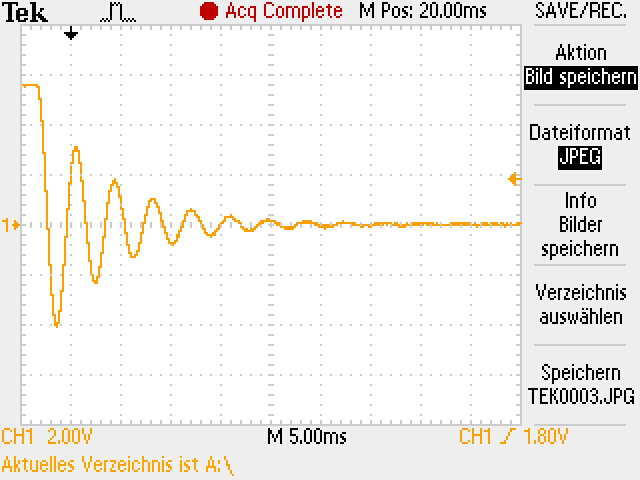
\includegraphics[scale=0.7]{TEK0003.JPG}
\caption{Beispiel: Messung 1}
\end{figure}


\newpage
\subsubsection{Transformation der Rohdaten}
Die Frequenzen wurden aus den Differenzen der Zeitabstände $T_i$ bestimmt. Bestimmung von Delta siehe Gleichung (\ref{Peter}). \\
Beispiel:

\begin{table}[H]\centering
\caption{Messung 1}
\begin{tabular}{c|c|c|c}
Frequenz in Hz & $\sigma_f$ in Hz & Abklingkoeffizient in $\frac{1}{s}$ & $\sigma_{\delta}$ in $\frac{1}{s}$\\ 
\hline
$f=256.410$& $\sigma_f=1.898$& $\delta=150.047$& $\sigma_{\delta}=4.264$\\ 
$f=263.158$& $\sigma_f=1.999$& $\delta=143.827$& $\sigma_{\delta}=7.260$\\
$f=263.158$& $\sigma_f=1.999$& $\delta=174.551$& $\sigma_{\delta}=13.535$\\
\end{tabular} 
\end{table}
Hier wurden die Fehler aus den folgenden Gleichungen ermittelt:
\begin{align}
\sigma_f&=\frac{\sigma_T}{T^2}\\
\sigma_{\delta_n}&=\frac{1}{T_n}\cdot \sqrt{(\frac{\sigma_{U_n}}{U_n})^2+(\frac{\sigma_{U_{n+1}}}{U_{n+1}})^2+(\delta_n\cdot \sigma_{T_n})^2}
\end{align}
Der Abklingkoeffizient $\delta$ wird bestimmt aus:

\begin{align}
U_{n+1}&=U_n \cdot e^{-\delta \cdot (t_{n+1}-t_n)}\notag \\
\Rightarrow \hspace{0.5cm} \delta_n&=\frac{\ln{\frac{U_n}{U_{n+1}}}}{t_{n+1}-t_n}
\label{Peter}
\end{align}
\newline
Aus den Einzelmessungen haben wir für die Frequenz und den Abklingkoeffizient den gewichteten Mittelwert mit seinem Fehler bestimmt:

\begin{table}[H]\centering
\caption{Ergebnis}
\begin{tabular}{c|c|c|c|c|c}
$\bar{f}$ in Hz & $\sigma_{\bar{f}}$ in Hz & $f_{Theo}$ & $\bar{\delta}$ in $\frac{1}{s}$ & $\sigma_{\bar{\delta}}$ in $\frac{1}{s}$& $\delta_{Theo}$ \\ 
\hline
$259.960$& $0.617$ & $264.426$ & $148.025$& $1.994$& $131.944$\\ 
\end{tabular} 
\end{table}

\begin{figure}[H]
\caption{Frequenz}
\centering
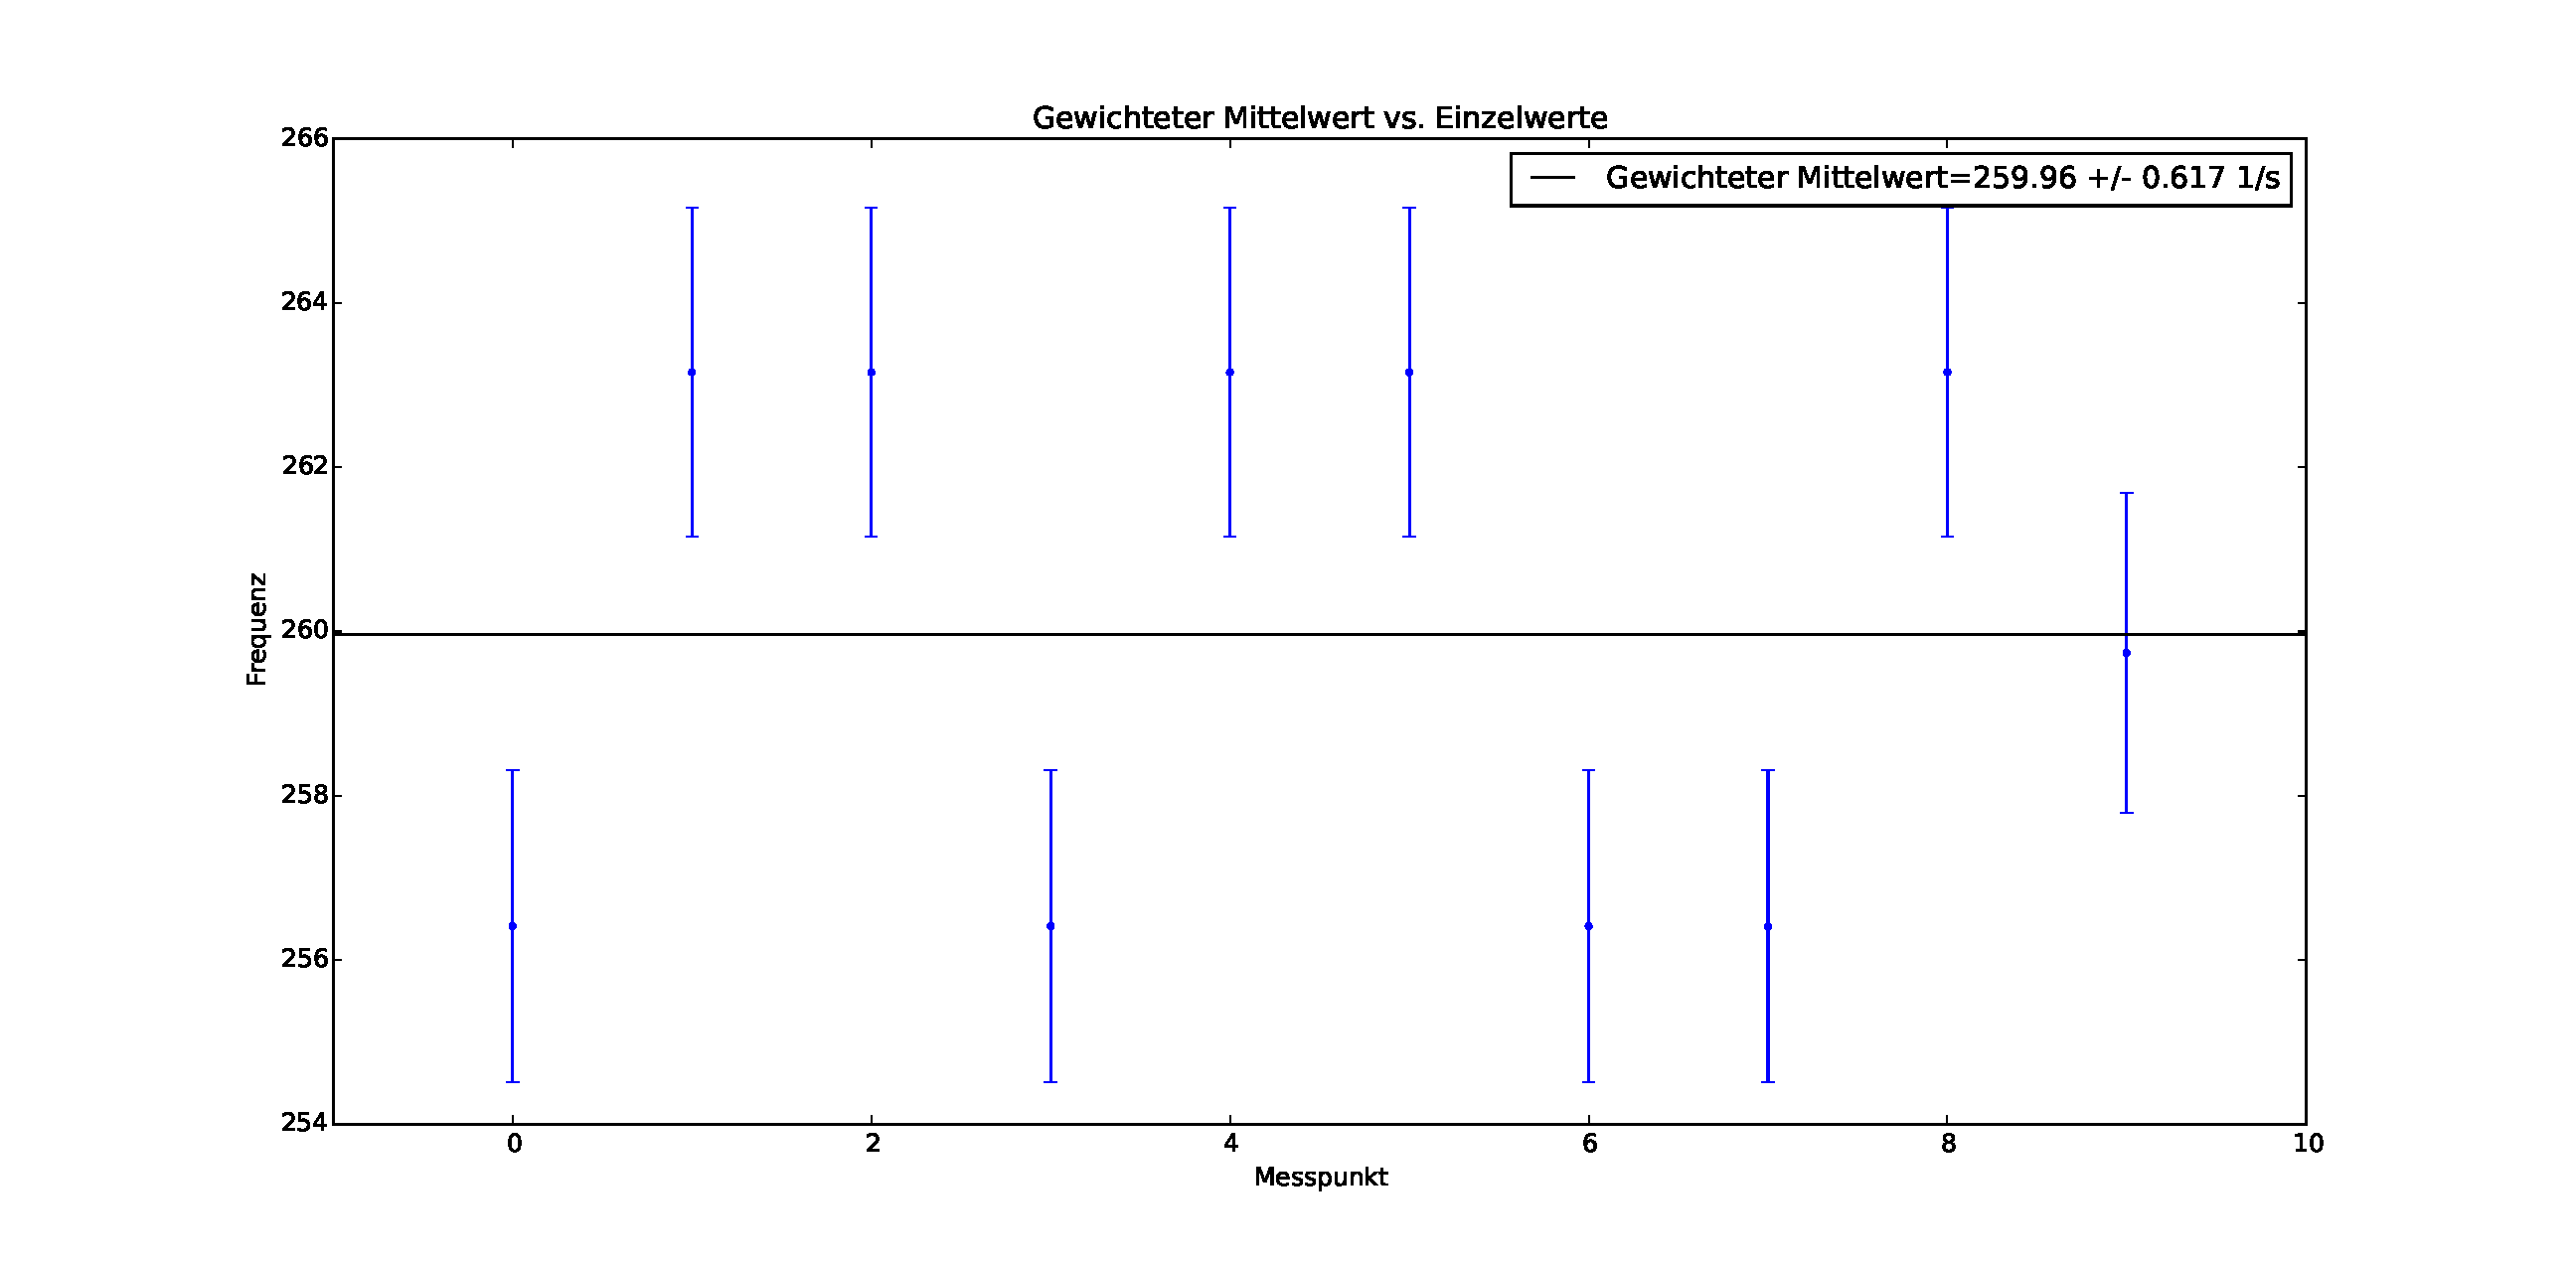
\includegraphics[scale=0.3]{Bilder/FrequenzGewichtet.eps}
\label{Frequenz_Oszi}
\end{figure}

\begin{figure}[H]
\caption{Abklingkoeffizient}
\centering
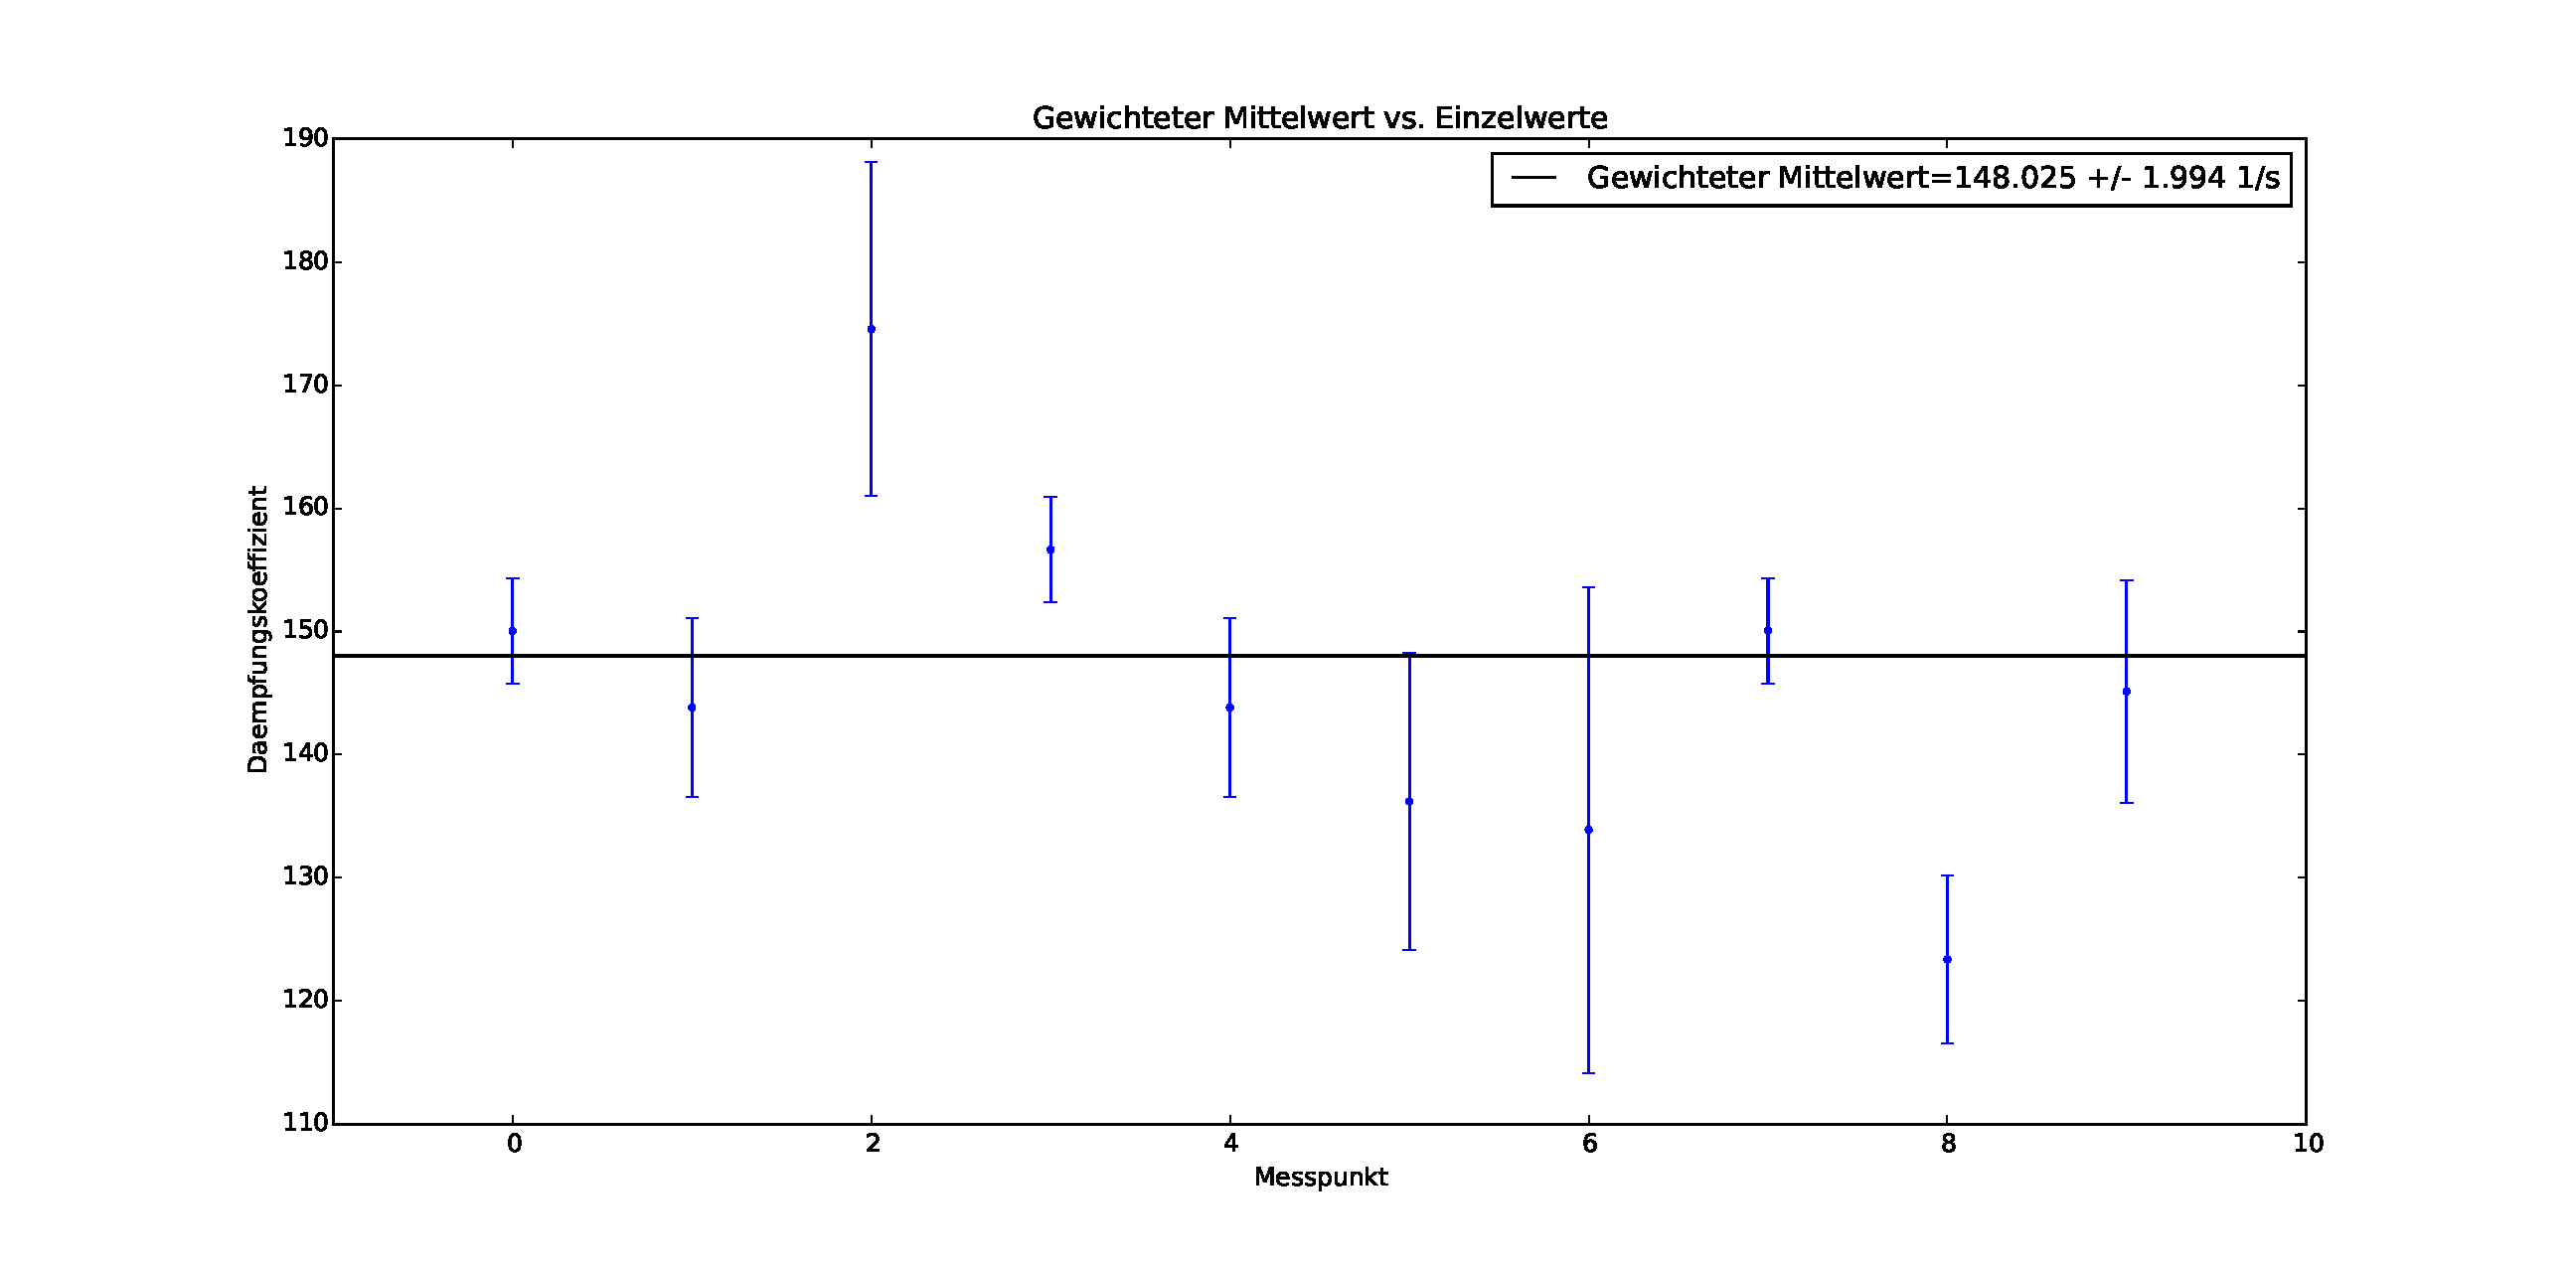
\includegraphics[scale=0.3]{Bilder/DaempfungGewichtet.eps}
\end{figure}


\subsubsection{Analyse und Fazit}
Auffällig ist, dass die gemessene Frequenz kleiner ist, als die theoretische Frequenz. Da die theoretische Frequenz allerdings allein aus den Herstellerangaben berechnet wurde ist ein ähnlicher Wert kaum zu erwarten. 
\newline
Weiterhin fällt auf, dass $\delta$ größer ist als $\delta_{theo}$. Der Grund dafür ist, dass $\delta \sim R$ und wir bei R mit Sicherheit einen höheren Wert erwarten müssten, da zum Beispiel alle Bauteile einen Innenwiderstand aufweisen. 
\newline
Die jeweiligen Fehler auf die Mittelwerte liegen in einem realistischen Rahmen.
\newline
Abbildung \ref{Frequenz_Oszi} zeigt einen zugegebenermaßen seltsamen Verlauf. Vier der Werte liegen auf extrem gleicher Höhe unter dem Graphen, fünf Werte auf ebenso gleicher Höhe über dem Graphen. Nur ein Fehlerbalken schneidet den Mittelwert. Wir erklären uns dies dadurch,  dass die gemessenen Zeitpunkte und deren Differenzen im Rahmen der Auflösung am Oszilloskop immer gleich waren (siehe Zeitmessung in Rohdaten).   
\newline
Erweitert man den Fehler auf $2\cdot\sigma$ ergibt sich, dass alle Fehler den Mittelwert schneiden.  
\begin{figure}[H]
\caption{Frequenz 2$\sigma$ }
\centering
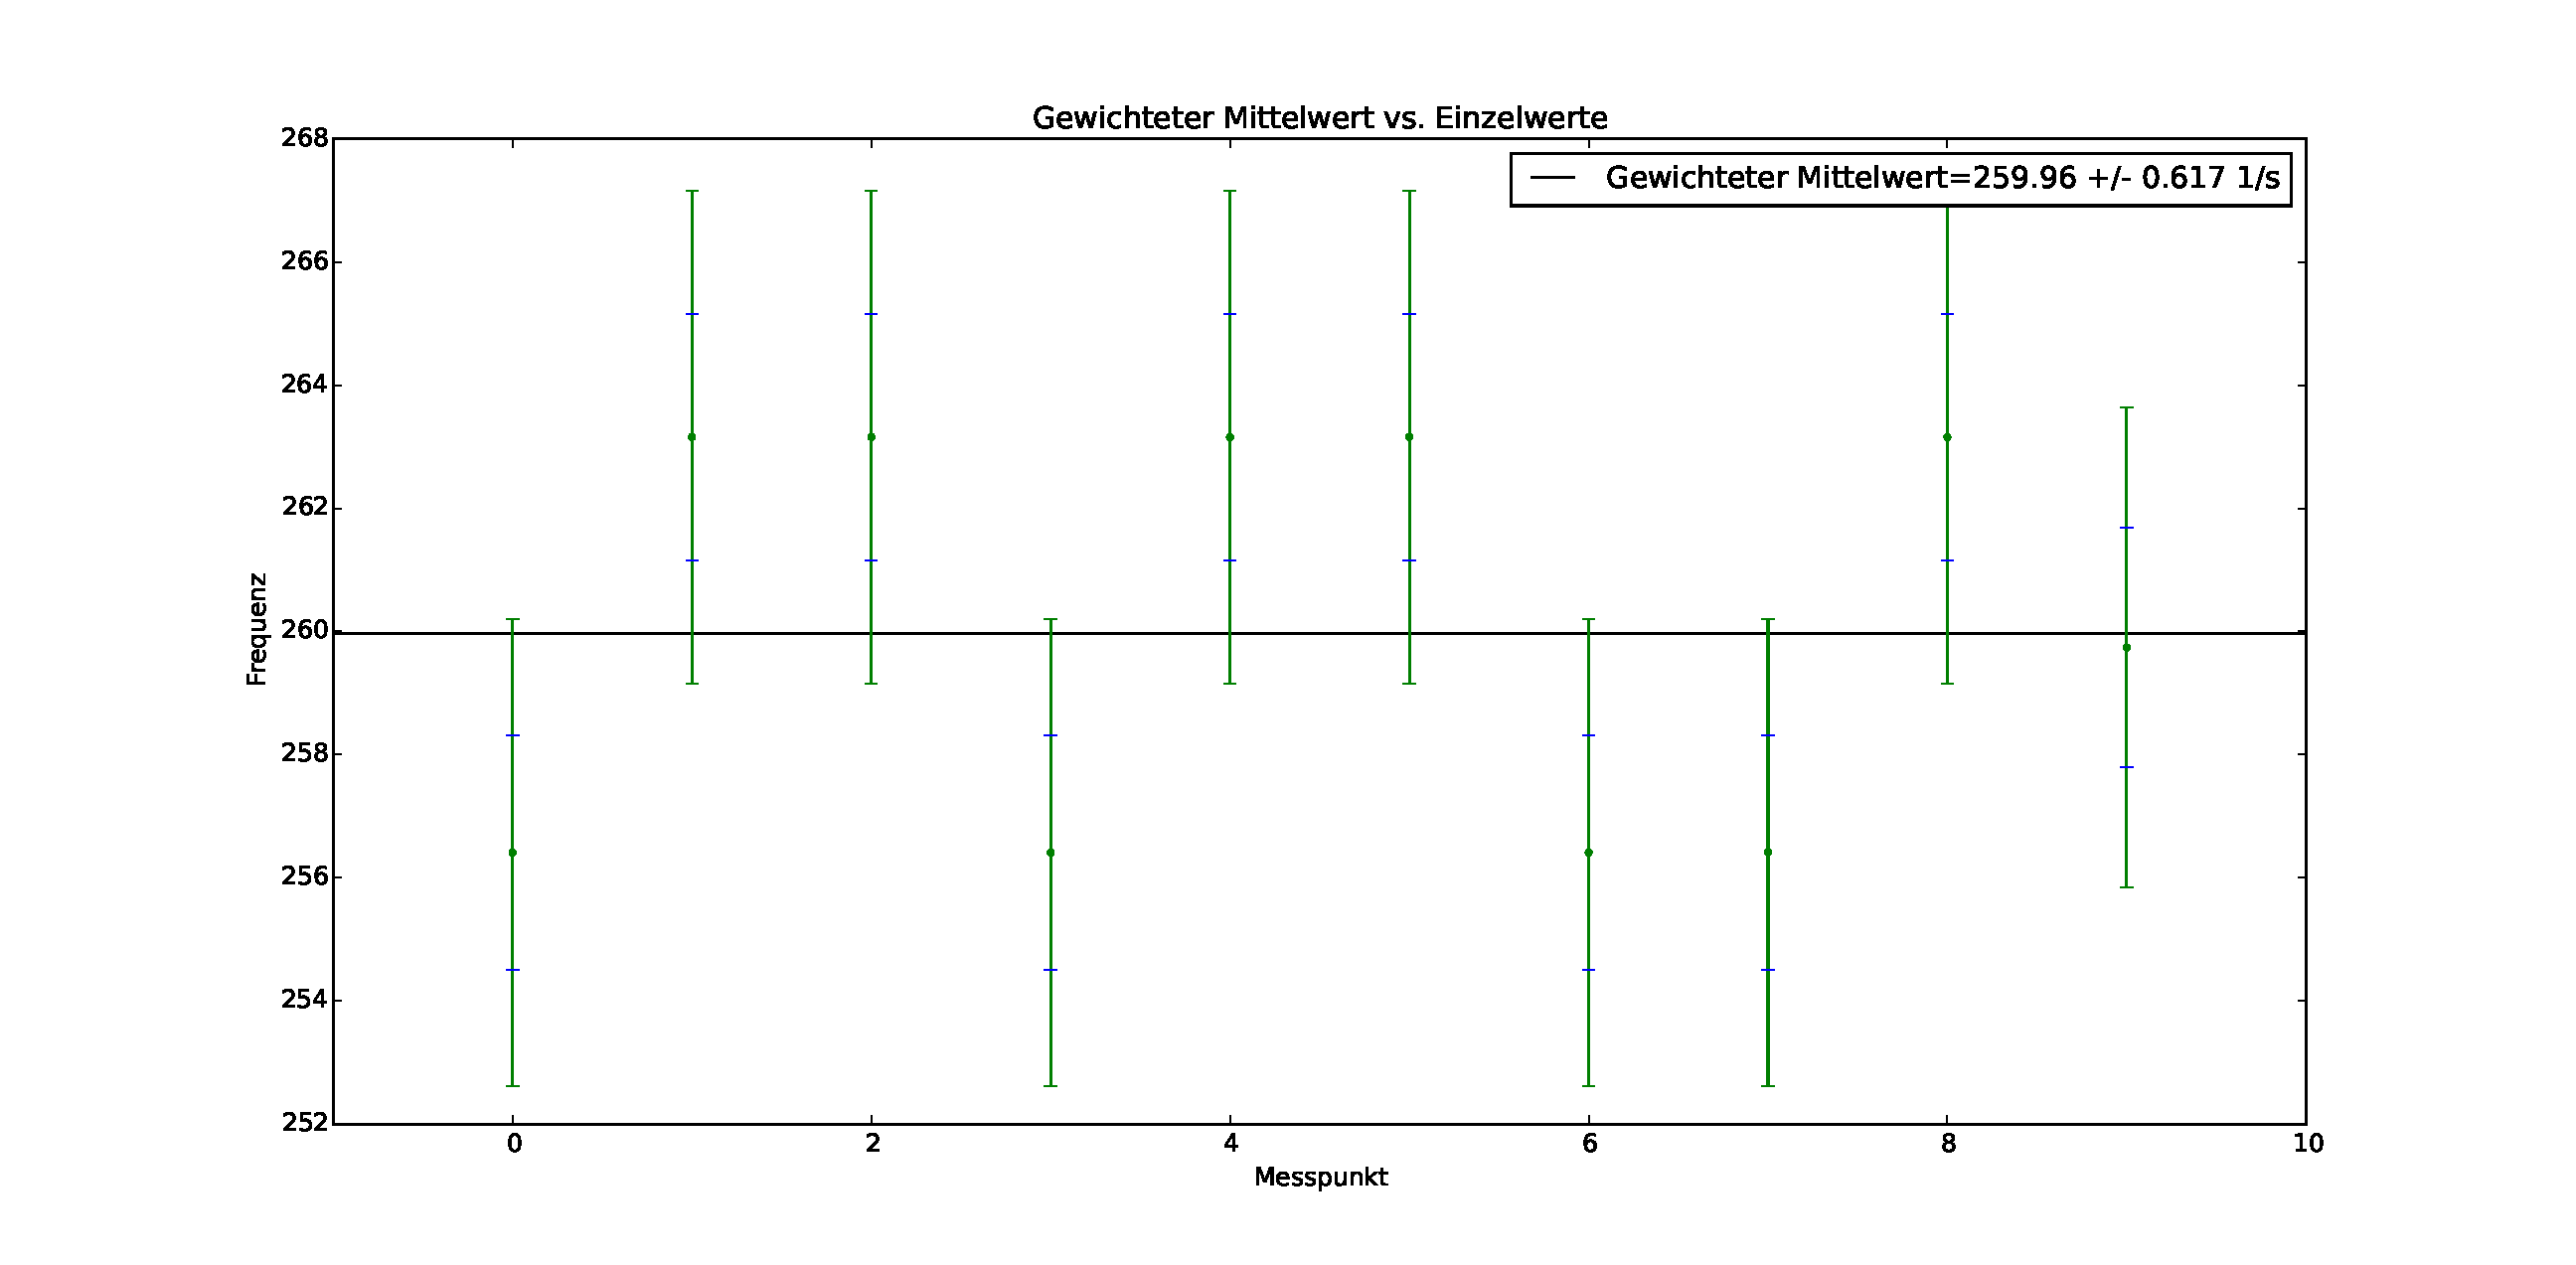
\includegraphics[scale=0.35]{Bilder/FrequenzGewichtetZweiSigma.eps}
\end{figure}

Der Plot zum Abklingkoeffizient sieht sehr vernünftig aus. Zwar schneiden nur 7 von 10 Fehlerbalken den Mittelwert, dies ist aber zu erwarten, da theoretisch nur $\approx 68\%$ der Werte den Mittelwert schneiden sollten.

\section{Gedämpfter LC Schwingkreis Cassy, Teilversuch 4.4.2}
\subsection{Versuchsbeschreibung}

Beim Teilversuch 4.4.2 sollte zunächst die Messung der Frequenz $f$ und die Messung des Dämpfungskoeffizienten $\delta$ wie in Teilversuch 4.4.1 wiederholt werden, nur dieses Mal sollte die Messung über das Sensor-Cassy statt über das Oszilloskop erfolgen.
Die Frequenz und der Dämpfungskoeffizient berechnen sich dabei nach den gleichen Formeln wie zuvor.
Die Schaltung sollte durch einen variierbaren Widerstand erweitert werden und mindestens ein Kriechfall($D=\frac{\delta}{\omega}>1$), ein Schwingfall($D<1$) und ein aperiodischer Grenzfall($D=1$) aufgenommen werden.
\newline
Nachdem die Dämpfungskonstante $\delta$ bestimmt wurde, konnte daraus die Induktivität der Spule über:
\begin{equation}
\delta =\frac{R}{2L} \hspace{1cm}
\Leftrightarrow  \hspace{1cm} L=\frac{1}{2\delta}\cdot R \label{Spule}
\end{equation}
bestimmt werden.
\newline
Für den aperiodischen Grenzfall gilt:
\begin{equation}
R_{ap}=2\cdot\sqrt{\frac{L}{C}}.
\label{aperiodischer GF}
\end{equation}
Dieser Grenzfall sollte mit Hilfe des Drehwiderstandes eingestellt und mit der Vorhersage verglichen werden.
\subsection{Versuchsaufbau}

Der Versuch wurde wie in der folgenden Skizze aufgebaut.

\begin{figure}[H]
    \subfigure[Versuchsaufbau aus dem Skript]{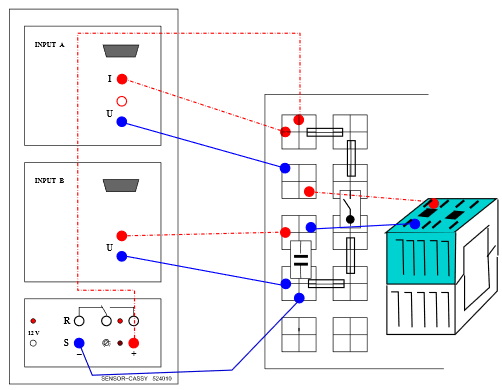
\includegraphics[width=0.49\textwidth]{Bilder/VersuchsaufbauOhneWiderstand.PNG}}
    \subfigure[unser Versuchsaufbau mit Widerstand]{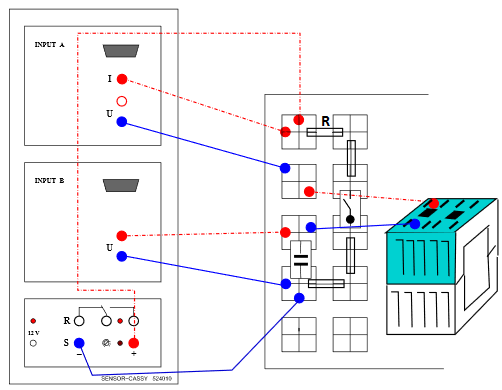
\includegraphics[width=0.49\textwidth]{Bilder/VersuchsaufbauMitWiderstand.PNG}}
\caption{Versuchsaufbau}
\end{figure}

Dabei wurde die Schaltung aus Teilversuch 4.4.1 fast gänzlich übernommen. Lediglich wurde das Oszilloskop durch ein Sensor Cassy ersetzt. Die Werte für die Spule, den Kondensator und die Eingangsspannung entsprechen daher denen aus Teilversuch 4.4.1.
Der skizzierte Dreh-Widerstand wurde auch im Aufbau zuvor benutzt allerdings auf null ($\approx$ 0.02 $\Omega$) gedreht.
\newline
Die Messbereiche wurden folgendermaßen eingestellt:
\begin{equation}
U_B=\pm 10 V \hspace{1cm} T_B=40 ms.
\end{equation}
Da wir die Schwingung eines sich entladenden gedämpften LRC-Schwingkreises bei einer Eingangsspannung von etwa $5.62V$ gemessen haben, haben wir den Trigger der Spannungsmessung auf ab $5.5V$ fallend eingestellt.
\newline

\subsection{Durchführung}
Insgesamt haben wir 34 Einzelmessungen durchgeführt. 
Dabei haben wir für die Messung der Induktivität unterschiedliche Widerstände über den Drehwiderstand eingestellt und gemessen. Für die Messung der Frequenz und des Dämpfungskoeffizienten haben wir mehrere Schwingungen für den selben Widerstand gemessen. Bei weiteren Messungen haben wir die Messzeit extrem verlängert, um einen eventuellen Offset besser abzuschätzen.
\newline
\newline
Für die Aufzeichnung eines Kriechfalls haben wir den Drehwiderstand durch einen $1k\Omega$ Widerstand ersetzt. Damit konnte sichergestellt werden, dass $D\gg 1$ und somit ein Kriechfall vorliegt.
\newline
Für die Aufzeichnung des aperiodischen Grenzfalls haben wir zunächst den nötigen Widerstand über Gleichung \ref{aperiodischer GF} abgeschätzt. Bei den gegeben Werten für R und L gilt dann:
\begin{equation}
R_{ap}\approx 120\Omega.
\end{equation}
Der Drehwiderstand musste also in diesen Bereich eingestellt und beobachtet werden ob bei der Schwingung die entsprechende Charakteristik vorliegt.
\newline
Für die Messung von $f,\delta$ und $L$ wurden Schwingfälle benötigt. Daher wurden hier Widerstände eingestellt, die deutlich unter $R= 120\Omega$ liegen.

\begin{figure}[H]
\caption{Aufbau}
\centering
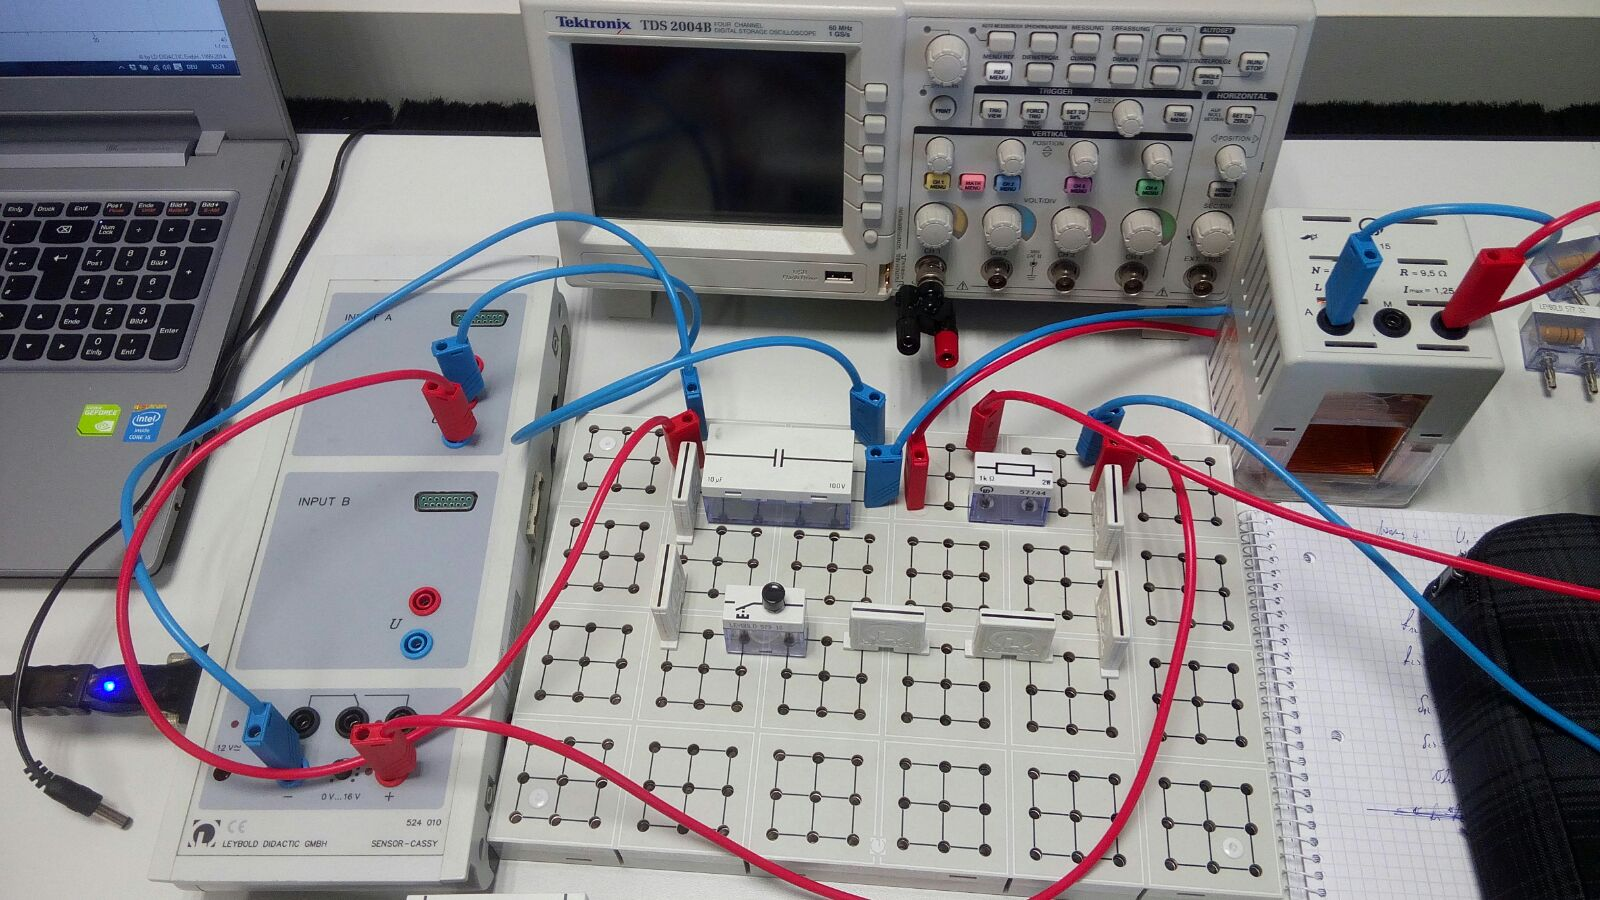
\includegraphics[scale=0.25]{Bilder/AufbauFoto.jpg}
\end{figure}



\newpage
\subsection{Versuchsauswertung}

\subsubsection{Rohdaten}
Bei der Vermessung mit dem Cassy wurde dieselbe Spule, derselbe Kondensator und dieselbe Eingangsspannung wie in Teilversuch 4.4.1 verwendet.

Aus der Auflösung des Cassy folgen Ablesefehler von:
\begin{equation}
\sigma_U=\frac{0.01V}{\sqrt{12}} \hspace{1cm}
\sigma_T=\frac{0.03ms}{\sqrt{12}}
\end{equation}

Im Folgenden sind Beispielmessungen abgebildet.

\begin{figure}[H]
\caption{Schwingfall bei $R\approx 0.02\Omega$ mit Bestimmung des Offsets}
\centering
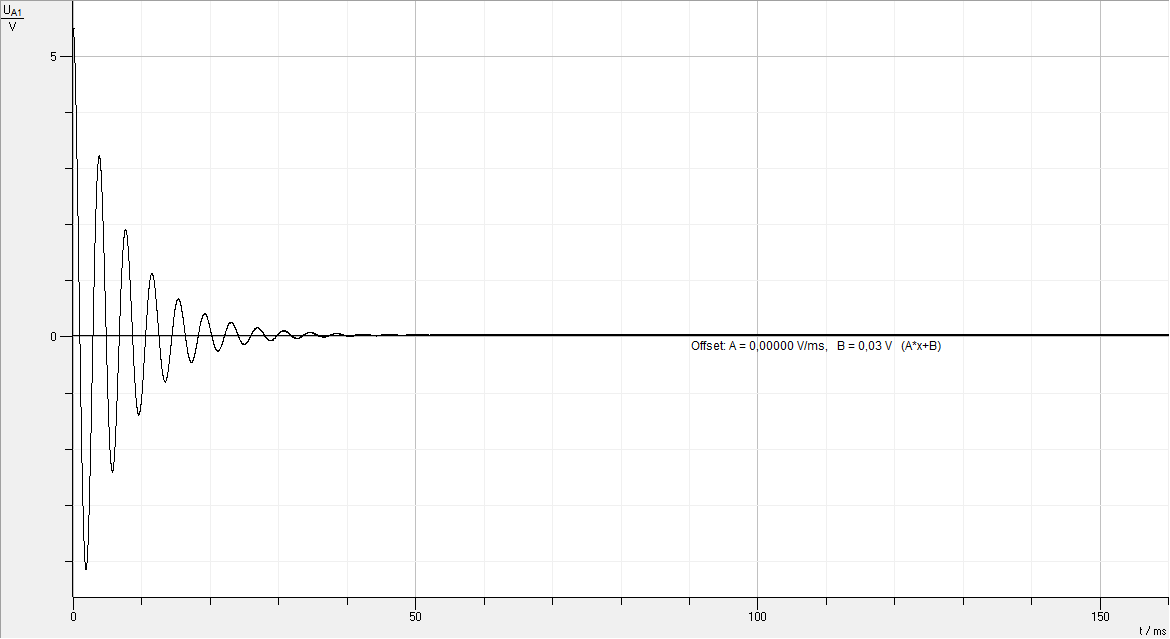
\includegraphics[scale=0.3]{Bilder/SchwingfallMitOffset0Ohm.png}
\end{figure}

\begin{figure}[H]
\caption{Schwingfall bei $2.4\Omega$}
\centering
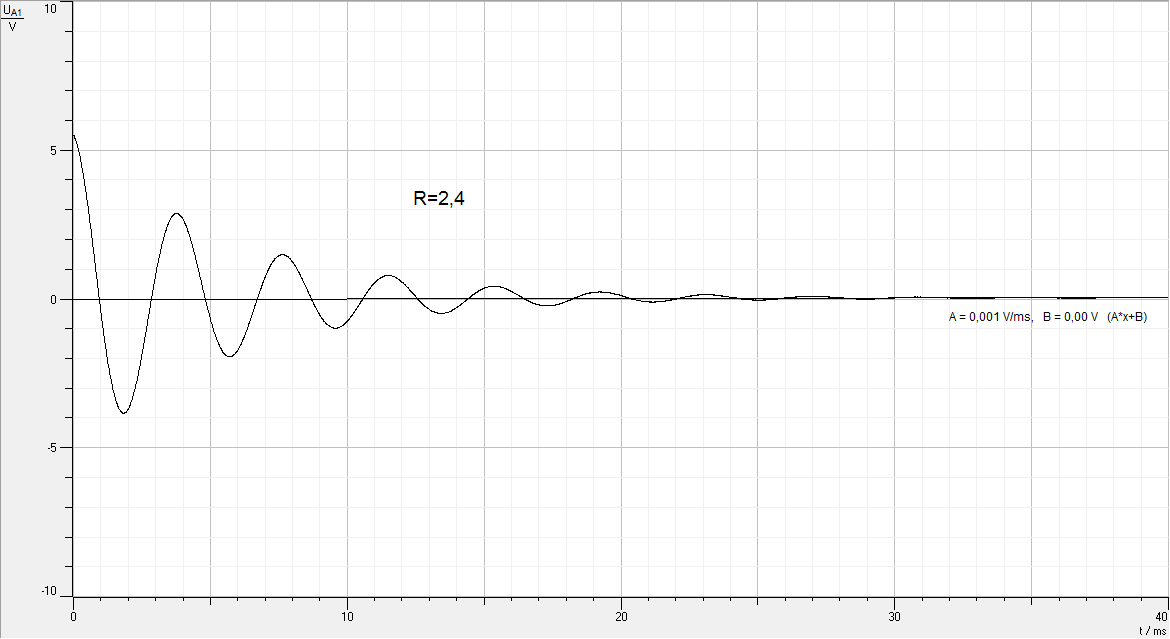
\includegraphics[scale=0.3]{Bilder/Schwingfall2komma4Ohm.png}
\end{figure}


\begin{figure}[H]
\caption{Kriechfall bei R=1k$\Omega$}
\centering
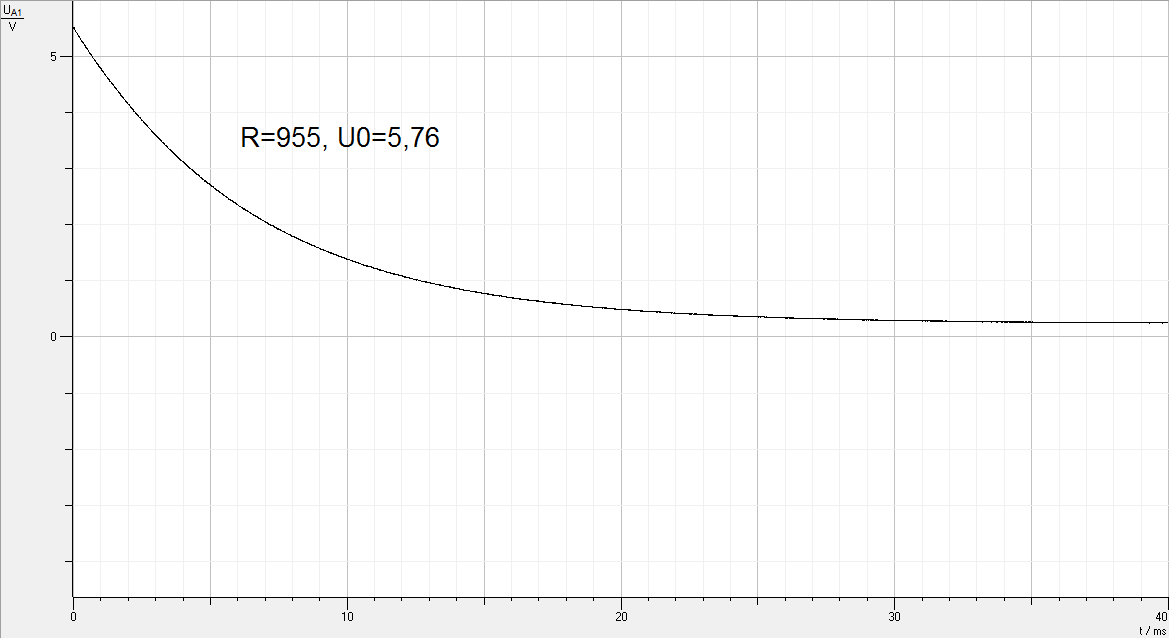
\includegraphics[scale=0.3]{Bilder/Kriechfall1KOhm.png}
\end{figure}




\subsubsection{Transformation der Rohdaten}
\textbf{Bestimmung der Frequenz durch FFT}: \\
Mithilfe der in Cassy eingebauten Fast-Fourier-Transformation(FFT) lässt sich sehr schnell die Frequenz einer Schwingung bestimmen:

\begin{figure}[H]
\caption{Bestimmung der Frequenz bei $R=2.4\Omega$ durch FFT}
\centering
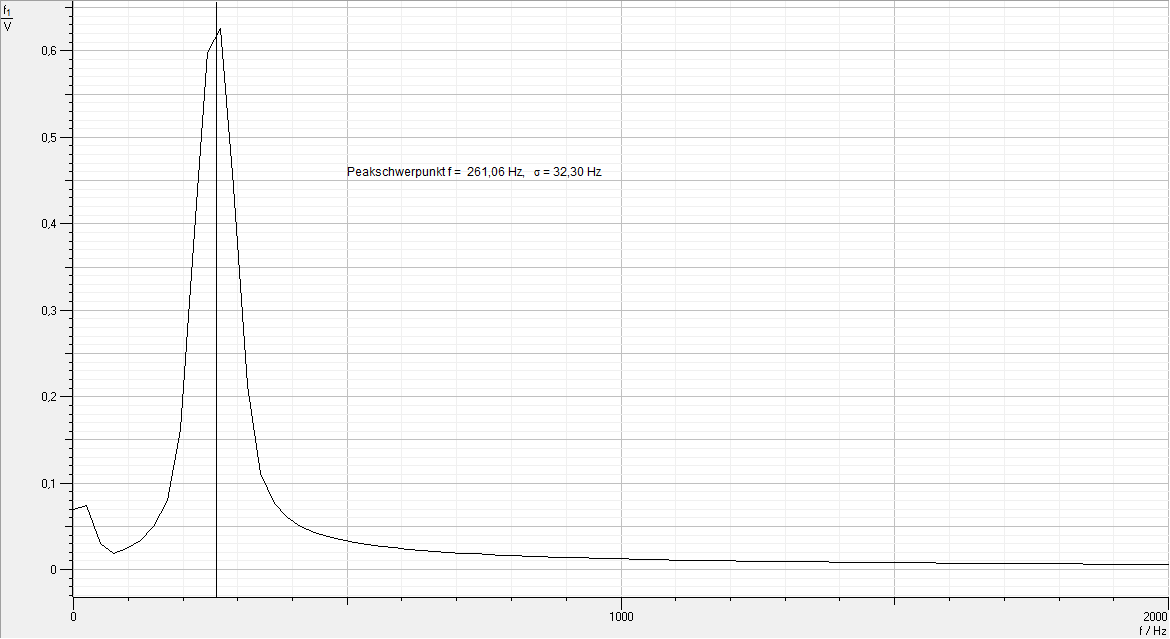
\includegraphics[scale=0.4]{Bilder/PEAK.png}
\end{figure}
\begin{equation}
f=261.06 Hz, \hspace{1cm} \sigma=32,3 Hz.
\end{equation}
Allerdings ist die Fehlerrechnung durch FFT fehlerhaft und undurchsichtig, die Fehlerabschätzung durch FFT ist also nicht sinnvoll. Im Folgenden haben wir die Frequenzen durch Ablesen bestimmt, um so auch den Fehler auf die Frequenz sinnvoll zu bestimmen.
\newline

\textbf{Bestimmung der Frequenz und des Dämpfungskoeffizienten durch Ablesen}: \newline
Wie bei Teilversuch 4.4.1 kann man die Frequenz und den Dämpfungskoeffizienten auch durch Ablesen der Maxima errechnen. Wichtig ist es auch hier den Offset vernünftig zu bestimmen und vor der Logarithmierung zu korrigieren.

\begin{figure}[H]
\caption{Messung der Minima und Maxima}
\centering
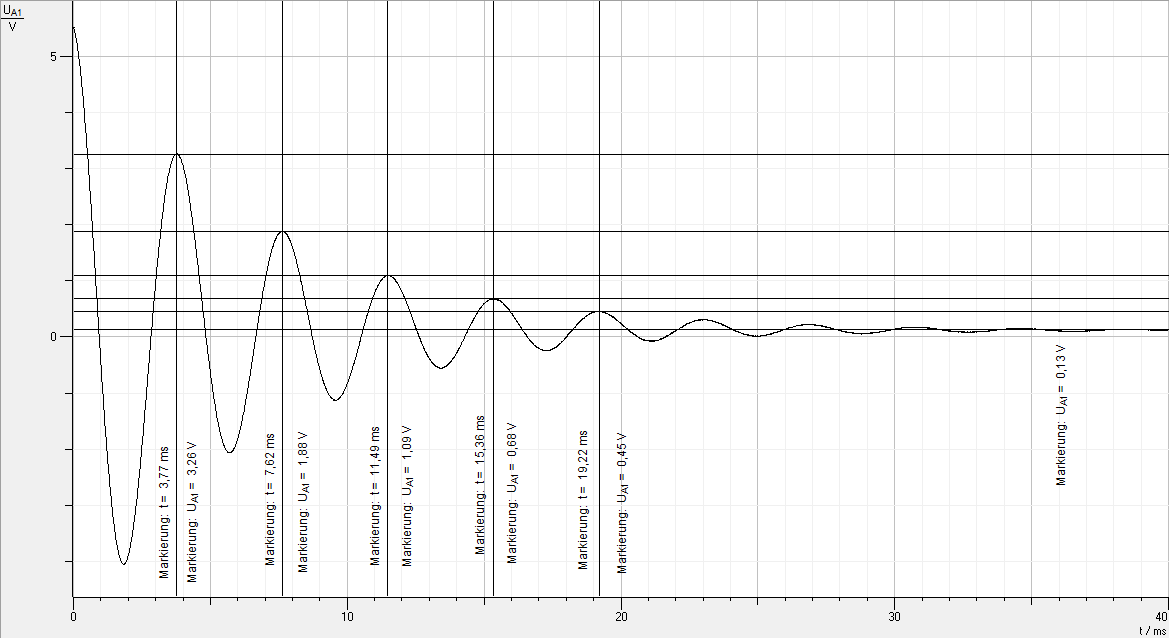
\includegraphics[scale=0.5]{Bilder/Einhuellende.png}
\end{figure}

Auf eben diese Weise haben wir 4 Schwingungen bei unterschiedlichen Widerständen vermessen.  Aus diesen Werten wurde jeweils die Frequenz und die Dämpfungskonstante mit Fehlern durch die Methode des gewichteten Mittelwerts bestimmt.\newline
Theoretisch können die Werte auch durch die Relationen:
\begin{align}
f_{Theo}&=\sqrt{\frac{1}{LC}-\frac{R^2}{4L^2}} \\
\delta_{Theo}&=\frac{R}{2L} 
\end{align}
bestimmt werden. \newline
Ergebnisse:
\begin{center}
\begin{tabular}{c|c|c|c|c|c|c}
R in $\Omega$ & $\bar{f}$ in Hz & $\sigma_{\bar{f}}$ in Hz & $f_{Theo}$ in Hz &  $\bar{\delta}$ in $\frac{1}{s}$ & $\sigma_{\bar{\delta}}$ in $\frac{1}{s}$  & $\delta_{Theo}$ in $\frac{1}{s}$ \\ 
\hline 
0.02 & 258.896 & 0.290 & 264.422 & 150.997 & 0.527 & 132.222 \\ 
\hline 
2.4 & 258.398 & 0.334 & 263.951 & 175.023 & 0.654  & 165.278\\ 
\hline 
5.5 & 257.046 & 0.331 & 263.178 & 225.027 & 1.050  & 208.333\\ 
\hline 
11.8 & 254.030 & 0.395 & 261.046 & 285.786 & 1.552  & 295.833 \\ 
\end{tabular} 
\end{center}

\textbf{Bestimmung der Induktivität}: \newline
Aus Relation (\ref{Spule}) folgt, dass die Steigung $a$ einer Geraden von $\delta$ gegen $R$, $a=\frac{1}{2L}$ entspricht.
Trägt man nun unsere Messwerte von $\delta$ unter Betrachtung der Fehler (Lineare Regression) gegen $R$ auf, ergibt sich der folgende Graph.
\begin{figure}[H]
\caption{Bestimmung der Induktivität mittels Linearer Regression}
\centering
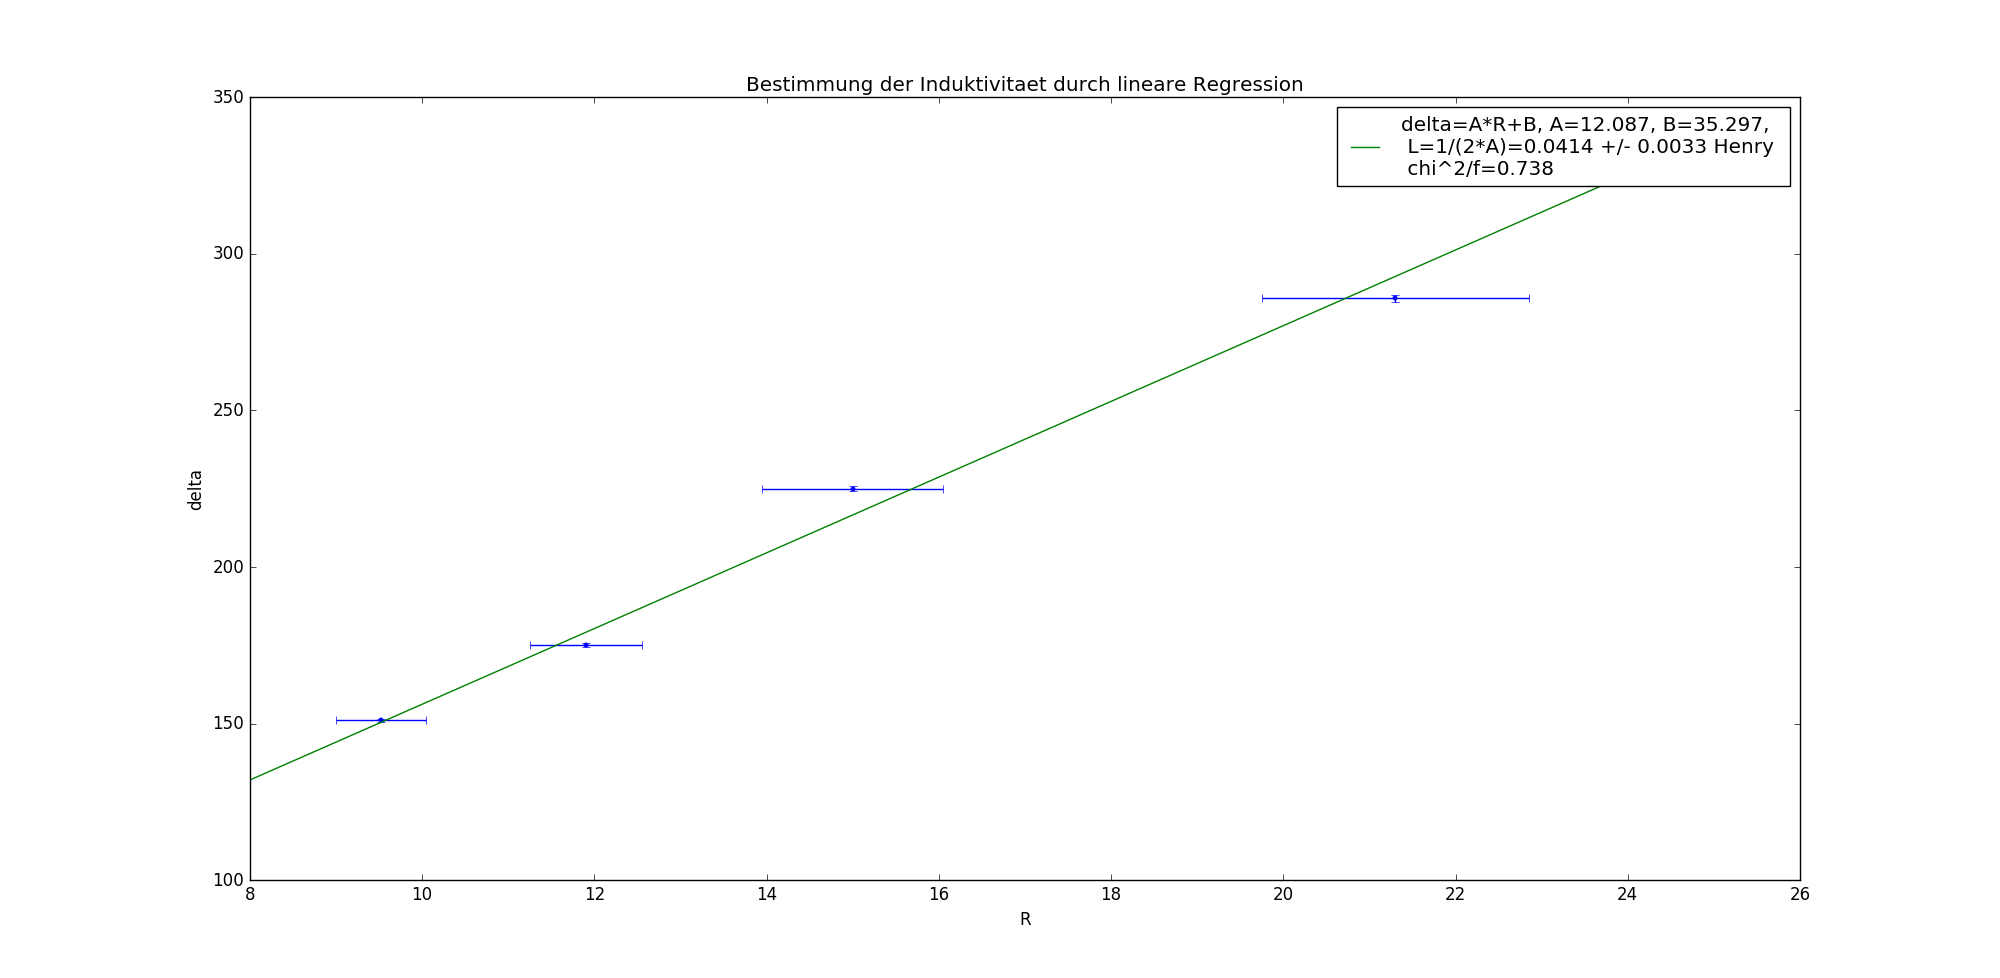
\includegraphics[scale=0.3]{Bilder/Induktivität_linreg.png}
\end{figure}
Der Fehler auf die Induktivität pflanzt sich dabei folgendermaßen fort:
\begin{equation}
\sigma_L=\frac{\sigma_A}{4A^2}
\end{equation}
Ergebnis:
\begin{align*}
\delta(R) &= A*R+B \\
A&=12.087 \frac{1}{H} \hspace{1cm} B=35.297 \frac{1}{s} \\
\Rightarrow L&=\frac{1}{2A}=0.0414 \pm 0.0033 H, \hspace{1cm} L_{Hersteller}=0.036 H\\
\frac{\chi^2}{f}&=0.738
\end{align*}




\subsubsection{Analyse und Fazit}
\textbf{Aperiodischer Grenzfall}
\begin{figure}[H]
\caption{Aperiodischer Grenzfall}
\centering
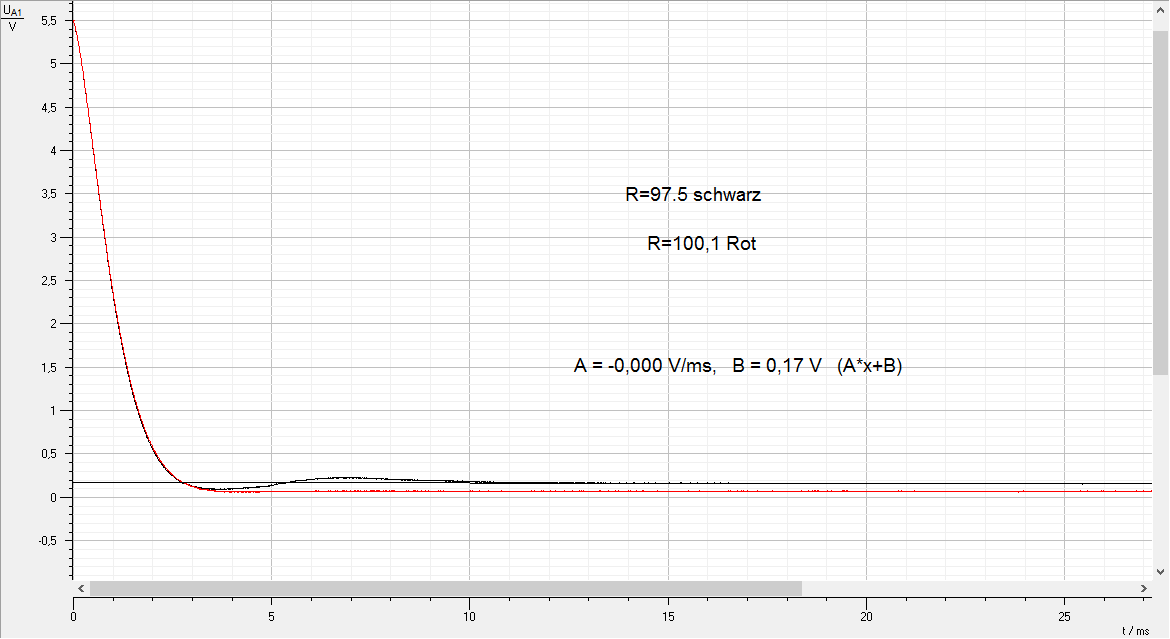
\includegraphics[scale=0.5]{Bilder/AperiodischerGrenzfall.png}
\label{Aperiodisch_Bild}
\end{figure}
Wie bereits erwähnt sollte der aperiodischer Grenzfall bei einem Widerstand von etwa
\begin{equation}
R_{ap}=2\cdot\sqrt{\frac{L}{C}}-R_{L}\approx 120\Omega - 9.5 \Omega=110.5\Omega
\end{equation}
aufteten. Mit $R_L$ dem Spuleninnenwiderstand.
Wie man in Abbildung \ref{Aperiodisch_Bild} sehr gut sieht schwingt die Schaltung bei $97.5\Omega$ noch, während sie bei $100.1\Omega$ gerade nicht mehr schwingt. Wir bestimmen den nötigen Widerstand für den aperiodischen Grenzfall also zu:
\begin{equation}
R_{ap}=100.1\Omega .
\end{equation}
Dieser Wert ist kleiner als der erwartete Wert, was aber zu erwarten war, da die Schaltung wahrscheinlich noch weitere Innenwiderstände hat als nur den auch sehr ungenauen Spuleninnenwiderstand.

\textbf{Analyse der Frequenz und des Dämpfungskoeffizienten durch Ablesen}: \newline
Betrachtet man die Frequenzen fällt auf, dass die berechneten kleiner sind als die theoretischen. Dies resultiert offenbar aus einem systematischen Fehler, denn die theoretischen Werte haben wir allein aus den Herstellerangaben für L, C und R berechnet. \newline
Der Fehler auf die Frequenz steigt mit steigendem R.
Dies kann man dadurch erklären, dass bei steigendem R die Dämpfung größer ist und somit weniger Maxima bzw. Messpunkte zur Verfügung standen.
\newline
Die Dämpfungskonstante steigt natürlich mit steigendem R, weil $\delta=\frac{R}{2L}\Rightarrow \delta \sim R$.
\newline
Diese Proportionalität pflanzt sich auch auf den Fehler von $\delta$ fort und erklärt somit auch das mit steigendem R steigende $\sigma_{\delta}$.


\textbf{Analyse der Induktivität}: \newline   
Bei der Linearen Regression kann man erkennen, dass  die Gerade alle Fehlerkästen schneidet. Der Fehler auf R ist dominant, was zu erwarten war, da wir ihn nur grob mit dem Drehwiderstand eingestellt und mit dem Multimeter überprüft haben (Fehlerabschätzung $\sigma_R=5\%$). 
\begin{figure}[H]
 \caption{Residuenplot für Induktivität}
 \centering
 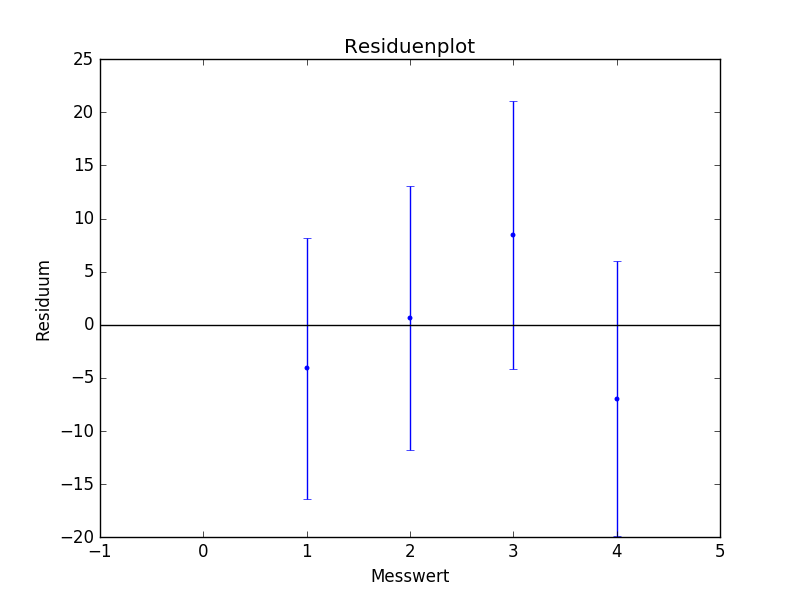
\includegraphics[scale=0.5]{Bilder/ResiduenplotInduktivitaeten.png}
\end{figure}
 
Der Residuenplot zeigt sowohl, dass keine Systematik vorliegt als auch, dass alle Werte mit ihren Fehlern passen. Auch das $\frac{\chi^2}{f}$ von $0.738$ ist passend. \newline

Der gemessene Wert für L ist kleiner als der theoretische. Dies lässt sich dadurch erklären, dass $L\sim R$ und wir wieder annehmen müssen, dass der Innenwiderstand  des gesamten Stromkreises als größer anzunehmen ist.

\textbf{Fazit}:\newline
Zusammenfassend kann man sagen, dass der Versuch äußerst erfolgreich verlaufen ist. Zwar weichen die gemessenen Werte oft von den theoretischen ab, die theoretischen Werte wurden allerdings auch nur aus den Herstellerangaben berechnet. Daher gehen wir davon aus, dass die von uns gemessenen Werte besser sind als die theoretischen.  


\end{document}